\documentclass[border=8pt]{standalone}
\usepackage[T1]{fontenc}\usepackage{helvet}\renewcommand{\familydefault}{\sfdefault}
\usepackage{tikz}\usetikzlibrary{arrows.meta, positioning, calc, backgrounds}
\definecolor{ink}{HTML}{1a1916}
\definecolor{inktwo}{HTML}{3a3a35}
\definecolor{inkthree}{HTML}{6a6862}
\definecolor{rule}{HTML}{b8b09a}
\definecolor{amber}{HTML}{a8730a}
\definecolor{red}{HTML}{c8261a}
\definecolor{paper}{HTML}{f0eee5}
\definecolor{slab}{HTML}{d8d4c6}
\tikzset{
  >={Stealth[length=2.2mm]},
  wire/.style={line width=0.8pt, ink},
  modwire/.style={line width=0.6pt, dashed, ink},
  tastewire/.style={line width=0.6pt, dashed, amber},
  gatewire/.style={line width=0.6pt, dotted, ink},
  block/.style={rectangle, draw=ink, line width=0.9pt, fill=slab, minimum width=2.4cm, minimum height=1.9cm, inner sep=0pt},
  perf/.style={rectangle, draw=ink, line width=0.7pt, minimum width=2.4cm, minimum height=0.7cm, inner sep=2pt, font=\footnotesize, text=ink},
  title/.style={font=\footnotesize\bfseries, text=ink, anchor=north, inner sep=2pt},
  jack/.style={circle, draw=ink, fill=paper, line width=0.5pt, minimum size=3.2pt, inner sep=0pt},
  plabel/.style={font=\tiny, text=inktwo, anchor=west, inner sep=1pt},
  olabel/.style={font=\tiny, text=inktwo, anchor=east, inner sep=1pt},
  settings/.style={font=\scriptsize, text=ink, align=left, anchor=north west, inner sep=1pt, text width=2.3cm},
}
\begin{document}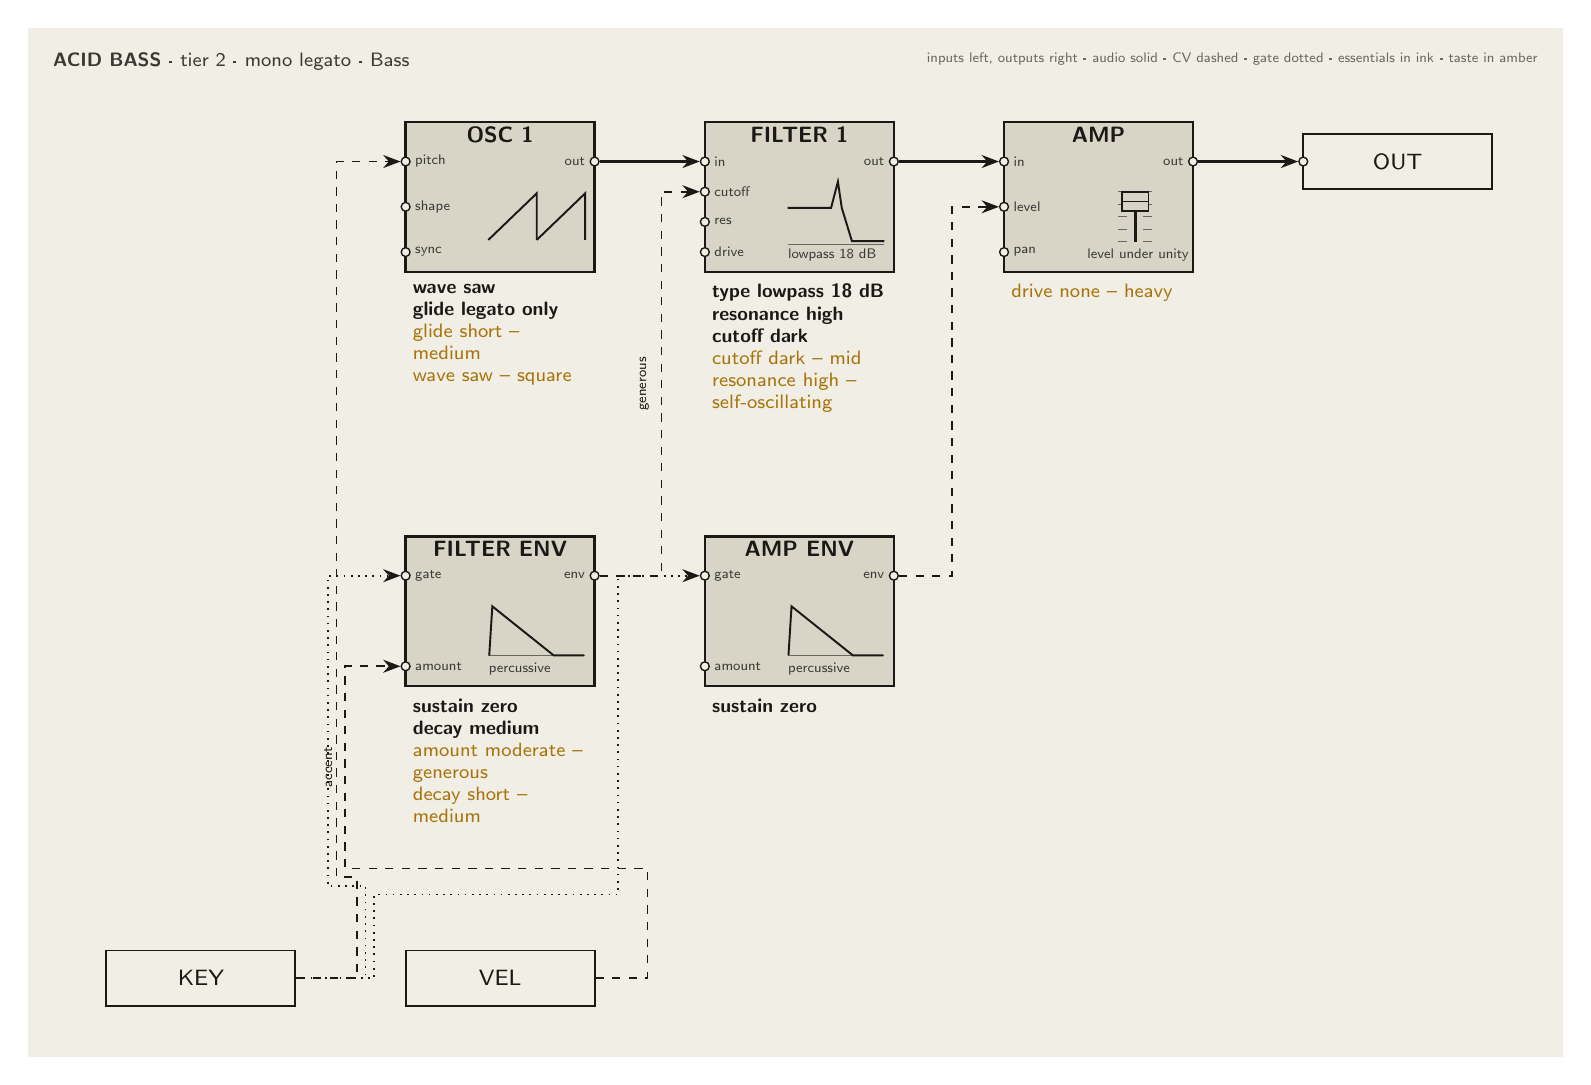
\begin{tikzpicture}
\begin{scope}[on background layer]\fill[paper] (-2.2,-10.92) rectangle (17.299999999999997,2.15);\end{scope}
\node[block, minimum height=1.9cm] (osc1) at (3.8,0.0) {};
\node[title] at (osc1.north) {OSC 1};
\node[jack] (osc1-pitch) at (2.5999999999999996,0.44999999999999996) {};
\node[plabel] at (2.6799999999999997,0.44999999999999996) {pitch};
\node[jack] (osc1-shape) at (2.5999999999999996,-0.125) {};
\node[plabel] at (2.6799999999999997,-0.125) {shape};
\node[jack] (osc1-sync) at (2.5999999999999996,-0.7) {};
\node[plabel] at (2.6799999999999997,-0.7) {sync};
\node[jack] (osc1-out) at (5.0,0.44999999999999996) {};
\node[olabel] at (4.92,0.44999999999999996) {out};
\begin{scope}
\draw[ink, line width=0.7pt] (3.650,-0.546) -- (4.265,0.046) -- (4.265,-0.546);
\draw[ink, line width=0.7pt] (4.265,-0.546) -- (4.880,0.046) -- (4.880,-0.546);
\end{scope}
\node[settings] at (2.6499999999999995,-1.0699999999999998) {\textbf{wave saw} \\ \textbf{glide legato only} \\ \textcolor{amber}{glide short -- medium} \\ \textcolor{amber}{wave saw -- square}};
\node[block, minimum height=1.9cm] (filter1) at (7.6,0.0) {};
\node[title] at (filter1.north) {FILTER 1};
\node[jack] (filter1-in) at (6.3999999999999995,0.44999999999999996) {};
\node[plabel] at (6.4799999999999995,0.44999999999999996) {in};
\node[jack] (filter1-cutoff) at (6.3999999999999995,0.06666666666666665) {};
\node[plabel] at (6.4799999999999995,0.06666666666666665) {cutoff};
\node[jack] (filter1-res) at (6.3999999999999995,-0.31666666666666665) {};
\node[plabel] at (6.4799999999999995,-0.31666666666666665) {res};
\node[jack] (filter1-drive) at (6.3999999999999995,-0.7) {};
\node[plabel] at (6.4799999999999995,-0.7) {drive};
\node[jack] (filter1-out) at (8.799999999999999,0.44999999999999996) {};
\node[olabel] at (8.719999999999999,0.44999999999999996) {out};
\begin{scope}
\draw[inkthree, line width=0.3pt] (7.450,-0.605) -- (8.680,-0.605);
\draw[ink, line width=0.7pt] (7.450,-0.139) -- (8.003,-0.139) -- (8.090,0.194) -- (8.139,-0.139) -- (8.268,-0.561) -- (8.680,-0.561);
\node[font=\tiny, text=inktwo, anchor=north west, inner sep=0pt] at (7.450,-0.650) {lowpass 18 dB};
\end{scope}
\node[settings] at (6.449999999999999,-1.0699999999999998) {\textbf{type lowpass 18 dB} \\ \textbf{resonance high} \\ \textbf{cutoff dark} \\ \textcolor{amber}{cutoff dark -- mid} \\ \textcolor{amber}{resonance high -- self-oscillating}};
\node[block, minimum height=1.9cm] (amp) at (11.399999999999999,0.0) {};
\node[title] at (amp.north) {AMP};
\node[jack] (amp-in) at (10.2,0.44999999999999996) {};
\node[plabel] at (10.28,0.44999999999999996) {in};
\node[jack] (amp-level) at (10.2,-0.125) {};
\node[plabel] at (10.28,-0.125) {level};
\node[jack] (amp-pan) at (10.2,-0.7) {};
\node[plabel] at (10.28,-0.7) {pan};
\node[jack] (amp-out) at (12.599999999999998,0.44999999999999996) {};
\node[olabel] at (12.519999999999998,0.44999999999999996) {out};
\begin{scope}
\draw[ink, line width=1.2pt] (11.865,-0.570) -- (11.865,0.070);
\draw[inkthree, line width=0.3pt] (11.645,-0.570) -- (11.765,-0.570) (11.965,-0.570) -- (12.085,-0.570);
\draw[inkthree, line width=0.3pt] (11.645,-0.410) -- (11.765,-0.410) (11.965,-0.410) -- (12.085,-0.410);
\draw[inkthree, line width=0.3pt] (11.645,-0.250) -- (11.765,-0.250) (11.965,-0.250) -- (12.085,-0.250);
\draw[inkthree, line width=0.3pt] (11.645,-0.090) -- (11.765,-0.090) (11.965,-0.090) -- (12.085,-0.090);
\draw[inkthree, line width=0.3pt] (11.645,0.070) -- (11.765,0.070) (11.965,0.070) -- (12.085,0.070);
\fill[slab, draw=ink, line width=0.6pt] (11.695,-0.178) rectangle (12.035,0.062);
\draw[ink, line width=0.5pt] (11.695,-0.058) -- (12.035,-0.058);
\node[font=\tiny, text=inktwo, anchor=north west, inner sep=0pt] at (11.250,-0.650) {level under unity};
\end{scope}
\node[settings] at (10.25,-1.0699999999999998) {\textcolor{amber}{drive none -- heavy}};
\node[block, minimum height=1.9cm] (fenv) at (3.8,-5.26) {};
\node[title] at (fenv.north) {FILTER ENV};
\node[jack] (fenv-gate) at (2.5999999999999996,-4.81) {};
\node[plabel] at (2.6799999999999997,-4.81) {gate};
\node[jack] (fenv-amount) at (2.5999999999999996,-5.959999999999999) {};
\node[plabel] at (2.6799999999999997,-5.959999999999999) {amount};
\node[jack] (fenv-out) at (5.0,-4.81) {};
\node[olabel] at (4.92,-4.81) {env};
\begin{scope}
\draw[inkthree, line width=0.3pt] (3.650,-5.821) -- (4.880,-5.821);
\draw[ink, line width=0.7pt] (3.662,-5.821) -- (3.701,-5.199) -- (4.479,-5.821) -- (4.479,-5.821) -- (4.868,-5.821);
\node[font=\tiny, text=inktwo, anchor=north west, inner sep=0pt] at (3.650,-5.910) {percussive};
\end{scope}
\node[settings] at (2.6499999999999995,-6.33) {\textbf{sustain zero} \\ \textbf{decay medium} \\ \textcolor{amber}{amount moderate -- generous} \\ \textcolor{amber}{decay short -- medium}};
\node[block, minimum height=1.9cm] (aenv) at (7.6,-5.26) {};
\node[title] at (aenv.north) {AMP ENV};
\node[jack] (aenv-gate) at (6.3999999999999995,-4.81) {};
\node[plabel] at (6.4799999999999995,-4.81) {gate};
\node[jack] (aenv-amount) at (6.3999999999999995,-5.959999999999999) {};
\node[plabel] at (6.4799999999999995,-5.959999999999999) {amount};
\node[jack] (aenv-out) at (8.799999999999999,-4.81) {};
\node[olabel] at (8.719999999999999,-4.81) {env};
\begin{scope}
\draw[inkthree, line width=0.3pt] (7.450,-5.821) -- (8.680,-5.821);
\draw[ink, line width=0.7pt] (7.462,-5.821) -- (7.501,-5.199) -- (8.279,-5.821) -- (8.279,-5.821) -- (8.668,-5.821);
\node[font=\tiny, text=inktwo, anchor=north west, inner sep=0pt] at (7.450,-5.910) {percussive};
\end{scope}
\node[settings] at (6.449999999999999,-6.33) {\textbf{sustain zero}};
\node[perf] (key) at (0.0,-9.92) {KEY};
\node[perf] (vel) at (3.8,-9.92) {VEL};
\node[perf, fill=paper] (out) at (15.2,0.44999999999999996) {OUT}; \node[jack] (out-in) at (14.0,0.44999999999999996) {};
\draw[wire,->] (osc1-out) -- (filter1-in);
\draw[wire,->] (filter1-out) -- (amp-in);
\draw[wire,->] (amp-out) -- (out-in);
\draw[modwire,->] (fenv-out) -- (5.85,-4.81) -- (5.85,0.06666666666666665) -- (filter1-cutoff);
\node[font=\tiny, text=ink, anchor=south, inner sep=1pt, rotate=90] at (5.7299999999999995,-2.3716666666666666) {generous};
\draw[modwire,->] (aenv-out) -- (9.54,-4.81) -- (9.54,-0.125) -- (amp-level);
\draw[modwire,->] (vel.east) -- (5.67,-9.92) -- (5.67,-8.530000000000001) -- (1.8299999999999998,-8.530000000000001) -- (1.8299999999999998,-5.959999999999999) -- (fenv-amount);
\node[font=\tiny, text=ink, anchor=south, inner sep=1pt, rotate=90] at (1.71,-7.245) {accent};
\draw[modwire,->] (key.east) -- (1.98,-9.92) -- (1.98,-8.64) -- (1.7199999999999998,-8.64) -- (1.7199999999999998,0.44999999999999996) -- (osc1-pitch);
\draw[gatewire,->] (key.east) -- (2.09,-9.92) -- (2.09,-8.75) -- (1.6099999999999999,-8.75) -- (1.6099999999999999,-4.81) -- (fenv-gate);
\draw[gatewire,->] (key.east) -- (2.2,-9.92) -- (2.2,-8.860000000000001) -- (5.3,-8.860000000000001) -- (5.3,-4.81) -- (aenv-gate);
\node[anchor=north west, font=\scriptsize, text=inktwo] at (-2.0,1.95) {\textbf{ACID BASS} · tier 2 · mono legato · Bass};
\node[anchor=north east, font=\tiny, text=inkthree] at (17.099999999999998,1.95) {inputs left, outputs right · audio solid · CV dashed · gate dotted · essentials in ink · taste in amber};
\end{tikzpicture}\end{document}
